\documentclass[a4paper,ngerman,landscape]{scrartcl}

\usepackage[utf8]{inputenc}

\usepackage[ngerman]{babel}
\usepackage{hyperref}

\usepackage{graphicx}
\usepackage{tikz}
\usetikzlibrary{calc}

\usepackage[protrusion=true,expansion=true]{microtype}

\usepackage{libertine}
\usepackage{tabto}

\setlength\parskip{\medskipamount}
\setlength\parindent{0pt}

\usepackage{geometry}
\geometry{tmargin=1.0cm,bmargin=1.0cm,lmargin=1.5cm,rmargin=1.5cm}

\pagestyle{empty}

\begin{document}

\begin{center}
  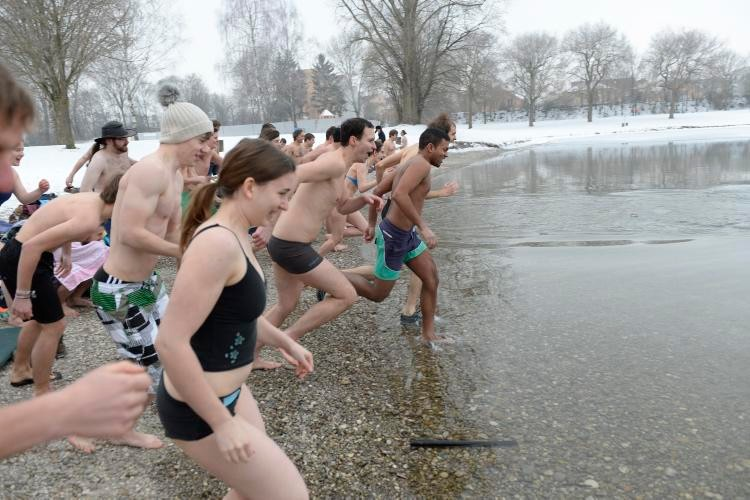
\includegraphics[height=0.15\textwidth]{eisbaden-7}
  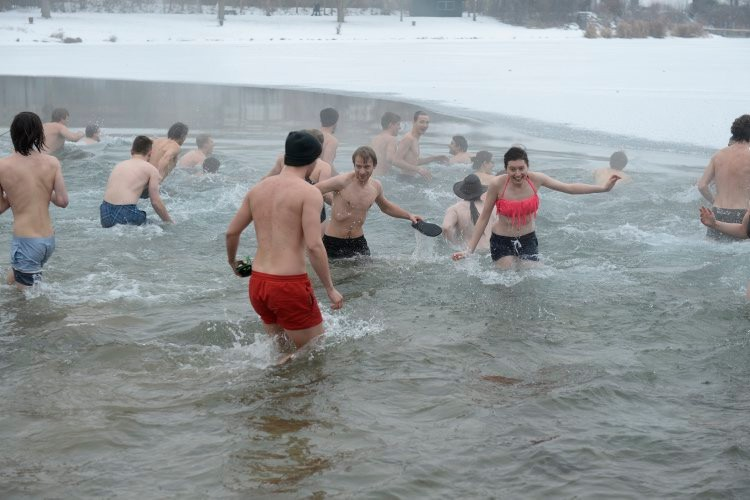
\includegraphics[height=0.15\textwidth]{eisbaden-5}
  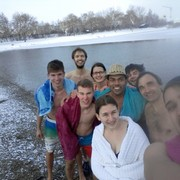
\includegraphics[height=0.15\textwidth]{eisbaden-1}
  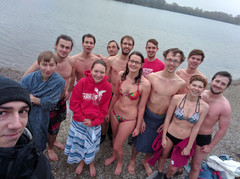
\includegraphics[height=0.15\textwidth]{eisbaden-2}
  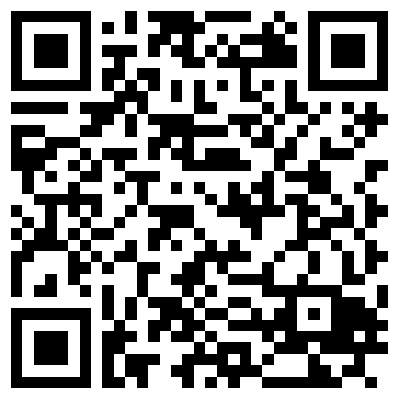
\includegraphics[height=0.15\textwidth]{eisbaden-qrcode6}
  \vspace{1em}

  \Huge
  \scalebox{3.4}{$\!\!$\textbf{\textcolor{red}{Neues} Eisbaden}}

  \large
  \begin{minipage}{0.92\textwidth}
    \renewcommand{\baselinestretch}{1.3}

    \setlength\parskip{\medskipamount}
    \vspace{0.3em}
    Eisbaden macht Spaß, tut gut und ist nicht so krass, wie man es sich vorstellt.
    Wir haben das schon oft gemacht, letztes Jahr mit fast
    50 Leuten. Wer Eisbaden also einmal ausprobieren möchte, ist herzlich
    eingeladen!
    Wir treffen uns am morgigen Mittwoch pünktlich um 15:45 Uhr bei der
    Schranke zwischen Mathe- und Info-Gebäude, um dann gemeinsam zum Ilsesee in
    Königsbrunn zu fahren. Um 16:40 Uhr sind wir wieder an der Uni.
    Wer mit möchte, muss sich nur auf \textsf{https:/$\!$/bit.ly/2Bec504} eintragen, damit
    wir die Anzahl Autos planen können.
    \vspace{0.3em}
  \end{minipage}

  \huge
  \scalebox{1.5}{Morgiger Mittwoch, 20. Dezember 2017, 15:45--16:40 Uhr}

  \tikz[remember picture,overlay] \node[opacity=1.0,inner sep=0pt] at (current
  page.south){\hspace*{-3cm}\vbox{\vspace*{-2.4cm}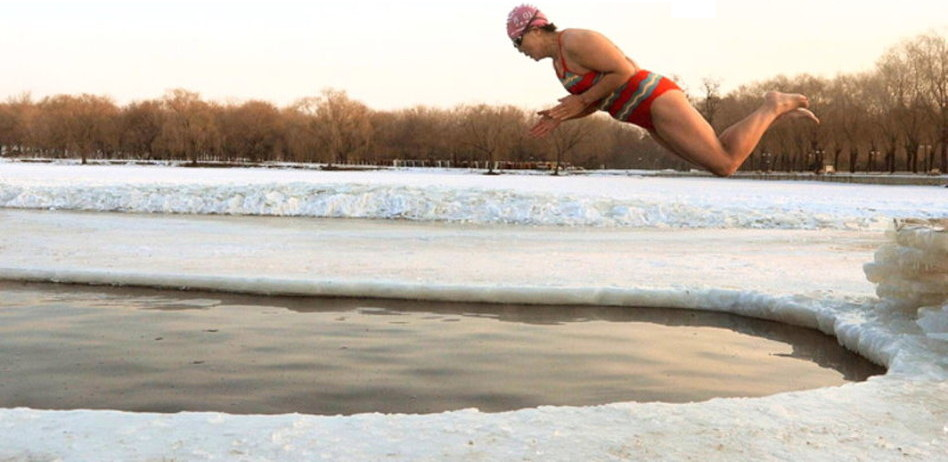
\includegraphics[width=\paperwidth]{eisbaden-sprung}}};
\end{center}

\end{document}
